% REPORT TEMPLATE
% Santiago Parraguez Cerda
% University of Chile 
% santiago.parraguez@ug.uchile.cl
%
% Version: 1.0.1 (08/08/2021)
% 
% CREATE DOCUMENT
\documentclass[a4paper, 11pt]{article} 
% Article size A4, 10pt (can be change to 'letterpaper' or any size you want).

% ============== DOCUMENT INFORMATION ====================
\newcommand{\reporttitle} {Report Title}
\newcommand{\maintopic} {Main topic}

\newcommand{\documentauthor} {Santiago Parraguez Cerda}
\newcommand{\coursename} {Name of the Course}
\newcommand{\coursecode} {ME710}

\newcommand{\universityname} {Universidad de Chile}
\newcommand{\facultyname} {Facultad del Ciencias Físicas y Matemáticas}
\newcommand{\universitydepartment} {Departamento de Ingeniería Mecánica}
\newcommand{\departmentimage} {/logos/dimec.pdf}
\newcommand{\departmentimageheight} {60pt}
\newcommand{\universitylocation} {Santiago, Chile}

% MEMBERS, TEACHERS and DATE
\newcommand{\tableofmembers} {
\begin{tabular}{ll}
	Estudiante:
	& \begin{tabular}[t]{l}
		Santiago Parraguez C.
	\end{tabular} \\
	Profesor:
	& \begin{tabular}[t]{l}
		Isaac Newton
	\end{tabular} \\
	%Auxiliar:
	%& \begin{tabular}[t]{l}
	%	Juneitor O.
	%\end{tabular} \\
	\multicolumn{2}{l}{Fecha de entrega: \today} \\
	\multicolumn{2}{l}{\universitylocation}
\end{tabular}}{
}
% ========================================================

% IMPORT CONFIGURATIONS
% ==================================
%      DOCUMENT CONFIGURATIONS
% ==================================

%% ------- GENERAL CONFIGURATION ----------
% Language (for babel)
\newcommand{\defaultlanguage} {english}
% Define default image folder
\newcommand{\defaultimagefolder} {img}
% Default interline distance
\newcommand{\defaultinterline} {1.0}
% Default new paragraph skip
\newcommand{\defaultparskip} {5pt}
% Default paragraph indentation
\newcommand{\defaultparindent} {17pt}
% Space before footnotes
\newcommand{\footnotespace}{15pt}
% Space between footnotes
\newcommand{\footnoteskip}{9pt}

% -------------- PAGE FORMAT --------------
% Portrait page top margin [cm]
\newcommand{\firstpagemargintop} {3.0}  
% Page top margin [cm]
\newcommand{\pagemargintop} {3.0}
% Page bottom margin [cm]
\newcommand{\pagemarginbottom} {2.7} 
% Page left margin [cm]
\newcommand{\pagemarginleft} {2.54}
% Page right margin [cm]
\newcommand{\pagemarginright} {2.54}

% -------------- PORTRAIT -----------------
% Header height of the portrait
\newcommand{\portraitheadheight} {70pt}

% -------------- INDEX --------------------
% Insert index
\newcommand{\showindex} {true}
% Show index of tables and figures
\newcommand{\showindextables} {true}
\newcommand{\showindexfigures} {true}
% Add a dot after numbers
\newcommand{\showdotafternum} {true}
% Skip before each section toc
\newcommand{\beforesecskip} {6pt}
% Skip before each subsection toc
\newcommand{\beforesubsecskip} {4pt}
% Skip before each subsubsection toc
\newcommand{\beforesubsubsecskip} {2pt}

% -------------- REFERENCES ---------------
% Sorting order of the references (nty, nyt, nyvt, anyt, anyvt, ydnt, none)
\newcommand{\biblatexsort} {nty}    
% Cite style (numeric, apa, authoryear, ieee)
\newcommand{\biblatexstyle} {apa}
% Max number of authors in apa configuration
\newcommand{\biblatexmaxapa} {99}
% Space between cite entries [pt]
\newcommand{\bibentrysep} {5pt}

% --------------- FLOAT OBJECTS -----------
% Indicate caption position, only for calculation. This does not mean that the caption is actually placed at top or bottom.
\newcommand{\tablecaptiontop} {true}
\newcommand{\figurecaptiontop} {false}
% Add section number to figures and tables
\newcommand{\fignumsec} {false}
\newcommand{\tabnumsec} {false}
% Figure default placement
\newcommand{\figureplacement}{htb}
% Table default placemente
\newcommand{\tableplacement}{htb}

% -------------- NAME OBJECTS -------------
% \newcommand{\nameabstract} {Abstracter}
\newcommand{\nametablecontents} {Table of Contents}
\newcommand{\namelisttables} {List of Tables}
\newcommand{\namelistfigures} {List of Figures}
\newcommand{\namereferences} {References}
% \newcommand{\namefigure} {Figurechan}
% \newcommand{\nametable} {Tablekun}
% \newcommand{\namesrc} {Source Codehack}
% \newcommand{\nameappendix} {Appendixix}


% IMPORT PACKAGES
% =================
%  PACKAGE IMPORTS
% =================
\usepackage[utf8]{inputenc}

\usepackage{array}
\usepackage{amsmath}
\usepackage{authblk}
\usepackage{booktabs}
\usepackage{caption}
\usepackage{csquotes}
\usepackage{fancyhdr}
\usepackage{geometry}
\usepackage{graphicx}
\usepackage{hyperref}
\usepackage{ifthen}
\usepackage{indentfirst}
\usepackage{lipsum}
\usepackage{microtype}
\usepackage{multirow}
\usepackage{ragged2e}
\usepackage{slantsc}
\usepackage{setspace}
\usepackage{titlesec}
\usepackage{xcolor}

% PACKAGE WITH CONFIGURATIONS
% ---------------------------
\usepackage[english]{babel}
\usepackage[shortlabels]{enumitem}

% CONDITIONAL PACKAGES
% --------------------
% BIBLATEX
\ifthenelse{\equal{\biblatexstyle}{apa}}{
    \usepackage[backend=biber, natbib, style=\biblatexstyle, sorting=\biblatexsort, uniquelist=false, apamaxprtauth=\biblatexmaxapa]{biblatex}
    }{
    \usepackage[backend=biber, natbib, style=\biblatexstyle, sorting=\biblatexsort, uniquelist=false]{biblatex}
}

% IMPORT COMMANDS
% =================
% TEMPLATE COMMANDS
% =================

% DEFINE ABSTRACT AND KEYWORDS
\renewcommand{\abstract}[1]{
    \def\theabstract{#1}
    }
\newcommand{\keywords}[1]{
    \def\thekeywords{#1}
    }
\newcommand{\corrauthor}[1]{
    \def\thecorrauthor{#1}
    }

% MAKETITLE COMMAND
\makeatletter
\renewcommand\maketitle{
    {\raggedright\LARGE\rmfamily\@title\\
    \vspace{0.5em}}
    \large\rmfamily\sffamily\@author\\
    \vspace{.1em} \hrule \vspace{1.2em}
    \normalfont
    \begin{tabular*}{\textwidth}{@{\extracolsep{\fill}} p{0.23\textwidth} @{} p{0.7\textwidth} @{}}
        \large{\textls[150]{\textsc{keywords}}} & \large{\textls[150]{\textsc{abstract}}} \\
        \addlinespace[0.4em]
        \cmidrule{1-1}\cmidrule{2-2}
        \addlinespace[0.25em]
        \raggedright\thekeywords & \theabstract \\
    \end{tabular*}
    \vspace{1.0em} \hrule \vspace{1.0em}
    }
\makeatother

% DEFINE NEW COLUMN TYPES FOR TABULAR
\newcolumntype{L}[1]{>{\raggedright\let\newline\\\arraybackslash\hspace{0pt}}m{#1}}
\newcolumntype{C}[1]{>{\centering\let\newline\\\arraybackslash\hspace{0pt}}m{#1}}
\newcolumntype{R}[1]{>{\raggedleft\let\newline\\\arraybackslash\hspace{0pt}}m{#1}}

% DEFINE TABLENOTE COMMAND
\newcommand{\tablenote}[2][-0.1em]{
    \renewcommand\arraystretch{100}
    \vspace{#1}\\{\footnotesize#2}
    }
    
% DEFINE BLIND FOOTNOTE
\newcommand\blfootnote[1]{%
    \begin{NoHyper}
    \renewcommand{\thefootnote}{}
    \footnotetext{#1}
    \renewcommand{\thefootnote}{\arabic{footnote}}
    \end{NoHyper}
}

% DEFINE PAGESTYLE
\fancypagestyle{core}{
	\fancyhf{}
	\rfoot{\thepage}
	\renewcommand{\headrulewidth}{0pt}
	\renewcommand{\footrulewidth}{0.4pt}
    }

% IMPORT INITIAL CONFIGURATION
% =================
%  DOCUMENT INIT
% =================

% CHANGE DEFAULT IMAGE FOLDER
\graphicspath{{./\defaultimagefolder}}

% Set page margins in cm (requires 'geometry')
\newcommand{\setpagemargincm}[4]{
    \newgeometry{left=#1cm, top=#2cm, right=#3cm, bottom=#4cm}
}

% RENEW AUTHOR AND AFFILIATION CONFIG
\renewcommand\Authfont{\normalfont}
\renewcommand\Affilfont{\slshape\footnotesize}
\renewcommand\Authsep{, }
\renewcommand\Authand{ and }
\renewcommand\Authands{ and }
\setlength{\affilsep}{.8em}

% FORMATTING SECTION TITLES
\titlelabel{\thetitle. }

\titlespacing*{\section}{0pt}{1.2ex plus .5ex minus .2ex}{.6ex plus .2ex}
\titlespacing*{\subsection}{0pt}{1.2ex plus .5ex minus .2ex}{.6ex plus .2ex}
\titlespacing*{\subsubsection}{0pt}{1.2ex plus .5ex minus .2ex}{.6ex plus .2ex}

% SET PARAGRAPH CONFIGURATIONS
\setlength{\parskip}{\setparskip}
\setlength{\parindent}{\setparindent}
\renewcommand{\baselinestretch}{\setbaselinestretch}

% INSERT REFERENCES
\addbibresource{references.bib}
\setlength{\bibhang}{1.5em}
\setlength{\bibitemsep}{.2em}
\renewcommand*{\bibfont}{\normalfont\small}

% CONFIGURE CAPTIONS
\captionsetup[table]{
    labelfont=bf, 
    labelsep=newline, 
    singlelinecheck=false, 
    skip=0.2\baselineskip
    }
\captionsetup[figure]{
    labelfont=bf, 
    singlelinecheck=false, 
    skip=0.4\baselineskip
    }
% \setlength\tabcolsep{0pt}

% SET COLOURS FOR LINKS
\definecolor{urlcolor}{rgb}{0.02, 0.27, 0.68}
\hypersetup{
    colorlinks=true,
    linkcolor=black,
    filecolor=cyan,
    citecolor=black,
    urlcolor=urlcolor
    }

% SET LIST CONFIGURATIONS
\setlist{itemsep=-0.2em}


% INSERT REFERENCES
\addbibresource{references.bib}

% ========================================================
\begin{document}
	
% PORTRAIT
% =========================
%      CREATE PORTRAIT
% =========================
\newpage
\setpagemargincm{\pagemarginleft}{\firstpagemargintop}{\pagemarginright}{\pagemarginbottom}

\thispagestyle{portrait}
	
~ \\
\vfill
\begin{center}
	{\noindent \huge{\coursecode \ \coursename\par}} ~ \\
    {\noindent \rule{\linewidth}{0.4mm}} ~ \\
	{\centering \noindent \Huge{\reporttitle\par}} ~ \\
    {\noindent \rule{\linewidth}{0.4mm}} ~ \\
	{\noindent \Large{\maintopic\par}}
\end{center}
\vfill

\vspace{1cm}
\noindent
\begin{minipage}{1.0\textwidth}
	\begin{flushright}
		\tableofmembers
	\end{flushright}
\end{minipage}
\vspace{1cm}

% ======================================
% CONFIGURE NEXT PAGES
\newpage
\setpagemargincm{\pagemarginleft}{\pagemargintop}{\pagemarginright}{\pagemarginbottom}
\pagestyle{prelude}
\setlength{\headheight}{20pt}
\pagenumbering{roman}
\setcounter{page}{1}

% ABSTRACT (you can erase it)
\begin{abstract}
    \lipsum[1]
\end{abstract}

% INSERT INDEX
% ======================
%      CREATE INDEX
% ======================
\renewcommand{\contentsname}{\nametablecontents}
\renewcommand{\listfigurename}{\namelistfigures}
\renewcommand{\listtablename}{\namelisttables}

\ifthenelse{\equal{\showindex}{true}}{

    \titlecontents{section} [2.0em] {\vspace{\beforesecskip}\normalfont\bfseries} {\contentslabel[\thecontentslabel.]{1.5em}} {\hspace*{-1.5em}}{\hfill\contentspage}
    \titlecontents{subsection} [5.0em] {\vspace{\beforesubsecskip}\normalfont} {\contentslabel[\thecontentslabel.]{2.5em}} {\hspace*{-2.5em}} {\titlerule*[10pt]{.}\contentspage}
    \titlecontents{subsubsection} [8.5em] {\vspace{\beforesubsubsecskip}\normalfont} {\contentslabel[\thecontentslabel.]{3.0em}} {\hspace*{-3.0em}} {\titlerule*[10pt]{.}\contentspage}
    
    \begingroup
    \clearpage
    \tableofcontents
    \clearpage
    \let\clearpage\relax
    \ifthenelse{\equal{\showindextables}{true}}{
        \listoftables}{}
    \ifthenelse{\equal{\showindexfigures}{true}}{
        \listoffigures}{}
    
    \endgroup
    \newpage
}{} 

% DOCUMENT PAGE CONFIGURATIONS
% ====================
%  PAGE CONFIGURATION
% ====================

% Set page margins
\setpagemargincm{\pagemarginleft}{\pagemargintop}{\pagemarginright}{\pagemarginbottom}

% Set column separation
\setlength{\columnsep}{\columnseparation}

% SET ABOVE AND BELOW DISPLAY SKIP
\setlength{\abovedisplayskip}{.5em}
\setlength{\belowdisplayskip}{1em}

% Make document two column and add title
\twocolumn[
\maketitle
]

% APPLY PAGE STYLE
\pagestyle{core}


% =========================== BEGIN DOCUMENT =========================

\section{Introducción}
% =========================================

\lipsum[1]


\section{Metodología}
% =========================================

\lipsum[2]

\subsection{No olvidar}

\lipsum[3] \citep{Chen2014}. Los resultados obtenidos se muestran en la Tabla \ref{tab:nombre_tabla}

\begin{table}[htb]
    \caption{Unos datos interesantes}
    \label{tab:nombre_tabla}
    \begin{tabular*}{\textwidth}{c @{\extracolsep{\fill}} l c r}
    \toprule
        A & B & C & D \\
    \midrule
        \multirow{2}{*}{E} & F & G & H \\
        & Como & Estás & ahi se nota mejor? \\
    \bottomrule
    \end{tabular*}
    \tablenote{Fuente: Elaboración propia. \lipsum[10]}
\end{table}

Quiero escribir un poco de texto, para saber como funciona el asuntito de poner una tabla. \lipsum[40]

\subsubsection{Aún tenemos más subsecciones}

\lipsum[4] \cite{Cengel2015} solo para probar \footnote{Aquí va un pie de página}. Además agregaré un segundo pie de página \footnote{Aquí escribimos otro}

\lipsum[9]

\subsubsection{Pongamos otra más}

\lipsum[5]

\lipsum[11]

\subsection{Y otra}

\lipsum[6] \footnote{Está bueno manejar estas distancias}

\begin{figure}[htb]
    \centering
    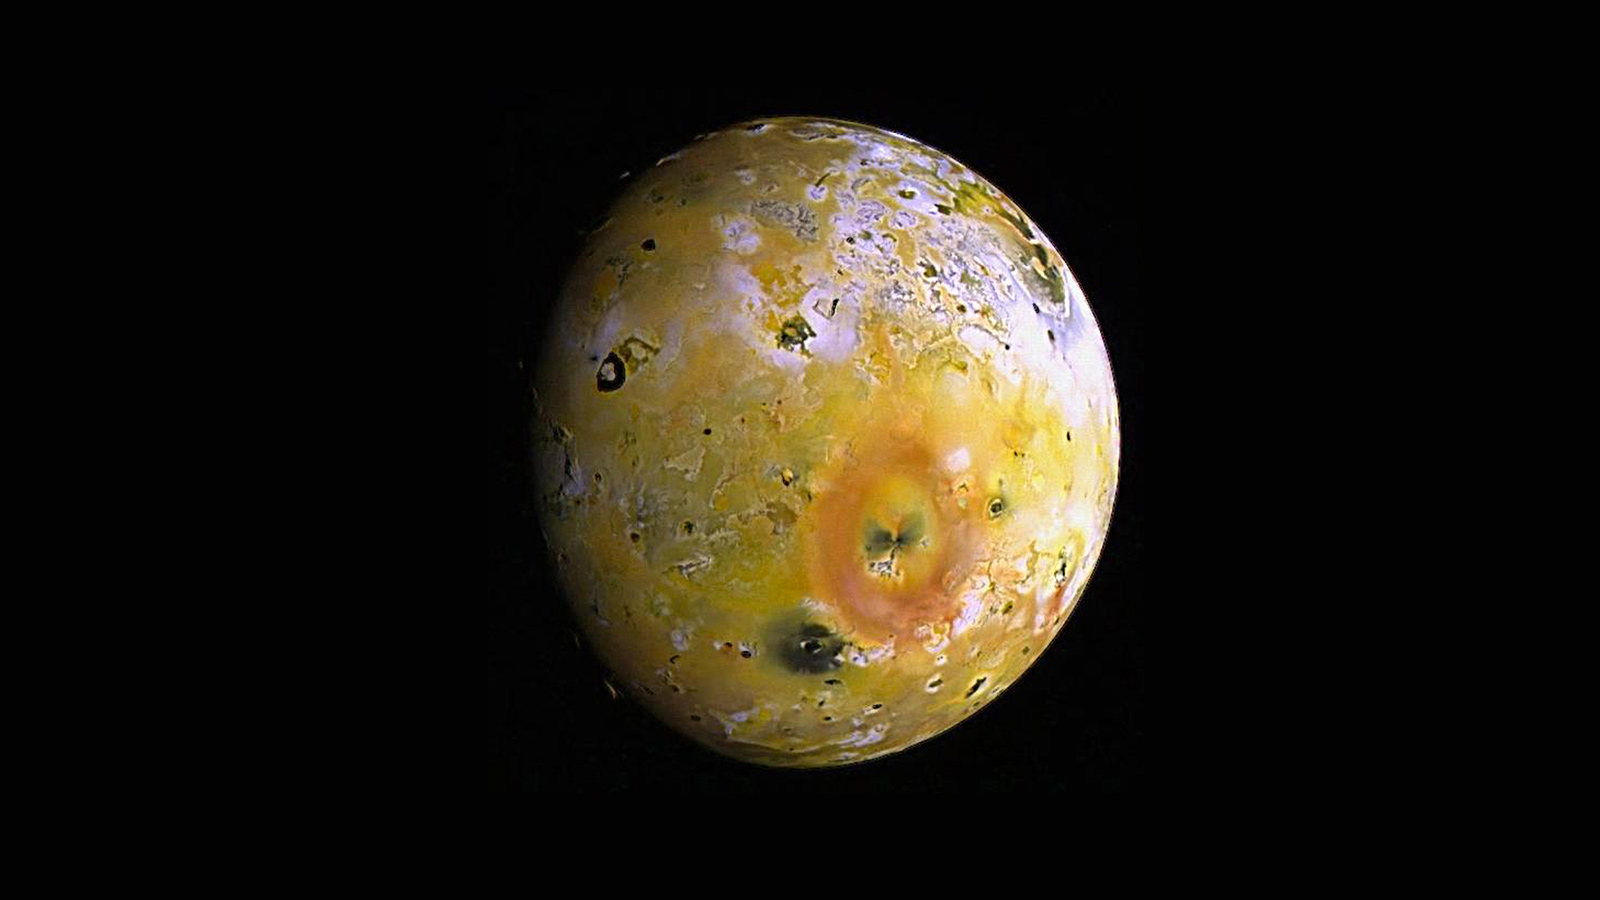
\includegraphics[width=0.6\textwidth]{img/giant-volcano-on-io-volcanic-moon-of-jupiter-expected-to-erupt.jpg}
    \caption{Io, luna de Júpiter seguiré escribiendo muchas cosas acá a ver qué pasa cuando me paso de la imagen. Debería ciertamente agregar variedad de palabrerío bastante extendido de manera que estafiguramuestremipunto}
    \label{fig:my_label}
\end{figure}

\lipsum[7]

\subsection{Y another}

\lipsum[8]

% ====================================================================
% REFERENCES
\newpage
\printbibliography[heading=bibintoc]

% END DOCUMENT
\end{document}